
\documentclass{article}

%%%%%%%%%%%%%%%%%%%%%%%%%%%%%%%%%%%%%%%%%
% Lachaise Assignment
% Structure Specification File
% Version 1.0 (26/6/2018)
%
% This template originates from:
% http://www.LaTeXTemplates.com
%
% Authors:
% Marion Lachaise & François Févotte
% Vel (vel@LaTeXTemplates.com)
%
% License:
% CC BY-NC-SA 3.0 (http://creativecommons.org/licenses/by-nc-sa/3.0/)
% 
%%%%%%%%%%%%%%%%%%%%%%%%%%%%%%%%%%%%%%%%%

%----------------------------------------------------------------------------------------
%	PACKAGES AND OTHER DOCUMENT CONFIGURATIONS
%----------------------------------------------------------------------------------------

\usepackage{amsmath,amsfonts,stmaryrd,amssymb} % Math packages

\usepackage{enumerate} % Custom item numbers for enumerations

\usepackage[ruled]{algorithm2e} % Algorithms

\usepackage[framemethod=tikz]{mdframed} % Allows defining custom boxed/framed environments

\usepackage{listings} % File listings, with syntax highlighting
\lstset{
	basicstyle=\ttfamily, % Typeset listings in monospace font
}

%----------------------------------------------------------------------------------------
%	DOCUMENT MARGINS
%----------------------------------------------------------------------------------------

\usepackage{geometry} % Required for adjusting page dimensions and margins

\geometry{
	paper=a4paper, % Paper size, change to letterpaper for US letter size
	top=2.5cm, % Top margin
	bottom=3cm, % Bottom margin
	left=2.5cm, % Left margin
	right=2.5cm, % Right margin
	headheight=14pt, % Header height
	footskip=1.5cm, % Space from the bottom margin to the baseline of the footer
	headsep=1.2cm, % Space from the top margin to the baseline of the header
	%showframe, % Uncomment to show how the type block is set on the page
}

%----------------------------------------------------------------------------------------
%	FONTS
%----------------------------------------------------------------------------------------

\usepackage[utf8]{inputenc} % Required for inputting international characters
\usepackage[T1]{fontenc} % Output font encoding for international characters

\usepackage{XCharter} % Use the XCharter fonts

%----------------------------------------------------------------------------------------
%	COMMAND LINE ENVIRONMENT
%----------------------------------------------------------------------------------------

% Usage:
% \begin{commandline}
%	\begin{verbatim}
%		$ ls
%		
%		Applications	Desktop	...
%	\end{verbatim}
% \end{commandline}

\mdfdefinestyle{commandline}{
	leftmargin=10pt,
	rightmargin=10pt,
	innerleftmargin=15pt,
	middlelinecolor=black!50!white,
	middlelinewidth=2pt,
	frametitlerule=false,
	backgroundcolor=black!5!white,
	frametitle={Command Line},
	frametitlefont={\normalfont\sffamily\color{white}\hspace{-1em}},
	frametitlebackgroundcolor=black!50!white,
	nobreak,
}

% Define a custom environment for command-line snapshots
\newenvironment{commandline}{
	\medskip
	\begin{mdframed}[style=commandline]
}{
	\end{mdframed}
	\medskip
}

%----------------------------------------------------------------------------------------
%	FILE CONTENTS ENVIRONMENT
%----------------------------------------------------------------------------------------

% Usage:
% \begin{file}[optional filename, defaults to "File"]
%	File contents, for example, with a listings environment
% \end{file}

\mdfdefinestyle{file}{
	innertopmargin=1.6\baselineskip,
	innerbottommargin=0.8\baselineskip,
	topline=false, bottomline=false,
	leftline=false, rightline=false,
	leftmargin=2cm,
	rightmargin=2cm,
	singleextra={%
		\draw[fill=black!10!white](P)++(0,-1.2em)rectangle(P-|O);
		\node[anchor=north west]
		at(P-|O){\ttfamily\mdfilename};
		%
		\def\l{3em}
		\draw(O-|P)++(-\l,0)--++(\l,\l)--(P)--(P-|O)--(O)--cycle;
		\draw(O-|P)++(-\l,0)--++(0,\l)--++(\l,0);
	},
	nobreak,
}

% Define a custom environment for file contents
\newenvironment{file}[1][File]{ % Set the default filename to "File"
	\medskip
	\newcommand{\mdfilename}{#1}
	\begin{mdframed}[style=file]
}{
	\end{mdframed}
	\medskip
}

%----------------------------------------------------------------------------------------
%	NUMBERED QUESTIONS ENVIRONMENT
%----------------------------------------------------------------------------------------

% Usage:
% \begin{question}[optional title]
%	Question contents
% \end{question}

\mdfdefinestyle{question}{
	innertopmargin=1.2\baselineskip,
	innerbottommargin=0.8\baselineskip,
	roundcorner=5pt,
	nobreak,
	singleextra={%
		\draw(P-|O)node[xshift=1em,anchor=west,fill=white,draw,rounded corners=5pt]{%
		Question \theQuestion\questionTitle};
	},
}

\newcounter{Question} % Stores the current question number that gets iterated with each new question

% Define a custom environment for numbered questions
\newenvironment{question}[1][\unskip]{
	\bigskip
	\stepcounter{Question}
	\newcommand{\questionTitle}{~#1}
	\begin{mdframed}[style=question]
}{
	\end{mdframed}
	\medskip
}

%----------------------------------------------------------------------------------------
%	WARNING TEXT ENVIRONMENT
%----------------------------------------------------------------------------------------

% Usage:
% \begin{warn}[optional title, defaults to "Warning:"]
%	Contents
% \end{warn}

\mdfdefinestyle{warning}{
	topline=false, bottomline=false,
	leftline=false, rightline=false,
	nobreak,
	singleextra={%
		\draw(P-|O)++(-0.5em,0)node(tmp1){};
		\draw(P-|O)++(0.5em,0)node(tmp2){};
		\fill[black,rotate around={45:(P-|O)}](tmp1)rectangle(tmp2);
		\node at(P-|O){\color{white}\scriptsize\bf !};
		\draw[very thick](P-|O)++(0,-1em)--(O);%--(O-|P);
	}
}

% Define a custom environment for warning text
\newenvironment{warn}[1][Warning:]{ % Set the default warning to "Warning:"
	\medskip
	\begin{mdframed}[style=warning]
		\noindent{\textbf{#1}}
}{
	\end{mdframed}
}

%----------------------------------------------------------------------------------------
%	INFORMATION ENVIRONMENT
%----------------------------------------------------------------------------------------

% Usage:
% \begin{info}[optional title, defaults to "Info:"]
% 	contents
% 	\end{info}

\mdfdefinestyle{info}{%
	topline=false, bottomline=false,
	leftline=false, rightline=false,
	nobreak,
	singleextra={%
		\fill[black](P-|O)circle[radius=0.4em];
		\node at(P-|O){\color{white}\scriptsize\bf i};
		\draw[very thick](P-|O)++(0,-0.8em)--(O);%--(O-|P);
	}
}

% Define a custom environment for information
\newenvironment{info}[1][Info:]{ % Set the default title to "Info:"
	\medskip
	\begin{mdframed}[style=info]
		\noindent{\textbf{#1}}
}{
	\end{mdframed}
}


\usepackage{hyperref}
\usepackage{url}

\usepackage[utf8]{inputenc}
\usepackage[T1]{fontenc}   
\usepackage{hyperref}      
\usepackage{url}           
\usepackage{booktabs}      
\usepackage{amsfonts}      
\usepackage{nicefrac}      
\usepackage{microtype}     
\usepackage{xcolor}        

\usepackage{array}
\usepackage{graphicx}
\usepackage{subfigure}
\usepackage{amsmath, bm}
\usepackage{dsfont}
\usepackage{amssymb}
\usepackage{multirow}
\usepackage{subcaption}
\usepackage{float}

\usepackage{varwidth}
\usepackage{pifont}
\usepackage{makecell}
\usepackage{wrapfig}
\usepackage{caption}
\usepackage{dsfont}
\usepackage{soul}
\usepackage[shortlabels]{enumitem}

\usepackage{pythonhighlight}

%----------------------------------------------------------------------------------------
%	ASSIGNMENT INFORMATION
%----------------------------------------------------------------------------------------

\title{EE379K: Assignment \#2}


\date{Due: Mar. 1 2024, 11:59pm TX}

%----------------------------------------------------------------------------------------

\begin{document}

\maketitle

%----------------------------------------------------------------------------------------
%	INTRODUCTION
%----------------------------------------------------------------------------------------

\section*{Introduction}

The overall goal of this homework is to implement a local feature matching algorithm. You can discuss in small groups, but turn in individual solutions and indicate collaborators. Turn in assignments by \textcolor{red}{Friday, Mar. 1}. Submit to Canvas a .zip file containing  (1) a questions.pdf with answers for Part 1 questions, (2) a writeup.pdf for Part 2 code; and (3) a \texttt{code/} directory containing your code without any large result files or subfolders. The pdf can be created using latex or converting a word document to pdf or any other method you prefer, as long as it is organized and easy to read. The submission template with latex and code for this homework can be found here: \href{https://classroom.github.com/a/mCG_ijF3}{https://classroom.github.com/a/mCG\_ijF3}.



\begin{info}
	\texttt{Szeliski} refers to the second edition of \textit{Computer Vision: Algorithms and Applications}, which can be found \href{http://szeliski.org/Book/}{here}.
\end{info}

%------------------------------------------------

\section{Part 1 Questions (30\%)}

\subsection*{Instructions}

\begin{itemize}
    \item Three graded questions.
    \item Write code where appropriate.
    \item Feel free to include images or equations.
    \item \textbf{We do NOT expect you to fill up each page with your answer.} Some answers will only be a few sentences long, and that is okay.
  \end{itemize}










\subsection{Q1} 
The Harris Corner Detector is commonly used in computer vision algorithms to find interest points from which to extract stable features for image matching. 

How do the eigenvalues of the `M' matrix change if we apply a low-pass filter to the image? What if we apply a high-pass filter? Describe qualitatively. 

Answer:
If we apply a low-pass filter to the image, the eigenvalues of the M matrix will \textbf{decrease}. This is because the low-pass filter will smooth the image, which will reduce the gradient magnitudes and thus the eigenvalues of the M matrix. The opposite is true for a high-pass filter, where the eigenvalues of the M matrix will \textbf{increase} because the high-pass filter will keep the high frequencies in the iamge, which will increase the gradient magnitudes and thus the eigenvalues of the M matrix.






\subsection{Q2} Given an interest point location, the SIFT algorithm converts a 16$\times$16 patch around the interest point into a 128$\times$1 feature descriptor of the gradient magnitudes and orientations therein. Write pseudocode \emph{with matrix/array indices} for these steps.


\emph{Notes} Do this for just one interest point at one scale; ignore the overall interest point orientation; ignore the Gaussian weighting; ignore all normalization post-processing; ignore image boundaries; ignore sub-pixel interpolation and just pick an arbitrary center within the 16$\times$16 for your feature descriptor. Please just explain in pseudocode how to go from the 16$\times$16 patch to the 128$\times$1 vector.
\begin{python}
    # You can assume access to the image, x and y gradients, and their magnitudes/orientations.
    image = imread('example.jpg')
    grad_x = filter(image, 'sobelX')
    grad_y = filter(image, 'sobelY')
    grad_mag = sqrt( grad_x .^2 + grad_y.^2 )
    grad_ori = atan2( grad_y, grad_x )
    
    # Takes in a interest point x,y location and returns a feature descriptor
    def SIFTdescriptor(x, y)
        descriptor = zeros(128,1)

        # loop through a 4x4 grid of 4x4 patches
        for i in range(-2, 2):
            for j in range(-2, 2):
                # i,j represents the 4x4 patch index
                patch_descriptor = zeros(8,1)
                for m in range(4):
                    for n in range(4):
                        # m,n represents the 4x4 pixel index
                        # get the gradient orientation and magnitude
                        grad_magnitude = grad_mag[x+i*4+m, y+j*4+n]
                        grad_orientation = grad_ori[x+i*4+m, y+j*4+n]
                        # convert the orientation to the 8-bin histogram index
                        bin_index = floor(grad_orientation // (pi/4))
                        # add the magnitude to the corresponding bin
                        patch_descriptor[bin_index] += grad_magnitude
                # add the 8-bin histogram to the descriptor
                descriptor.append(patch_descriptor)
        return descriptor
    \end{python}
    
\subsection{Q3} Distance metrics for feature matching.

\begin{enumerate}[(a)]
    \item Explain the differences between the geometric interpretations of the Euclidean distance and the cosine similarity metrics. What does this tell us about when each should be used?
    \item Given a distance metric, what is a good method for feature descriptor matching and why?
\end{enumerate}

Answer:
\textbf{Difference between Euclidean distance and cosine similarity: } The Euclidean distance measures the distance between two points in a space, while the cosine similarity measures the angle between two vectors. The Euclidean distance is sensitive to the magnitude of the vectors, while the cosine similarity is not. This means that the Euclidean distance will be large if the vectors are far apart in space and cosine similarity will be large is the direction of the vectors is vastly different. This tells us that the Euclidean distance should be used when the magnitude of the vectors is important, while the cosine similarity should be used when the direction of the vectors is important. 

\textbf{Good method for feature descriptor matching: } 

\section{Writeup}

\subsection{Notre Dame}
\begin{itemize}
    \item Image 1 - Number of interest points: 338
    \item Image 2 - Number of interest points: 291
    \item Matches: 156
    \item Accuracy on 50 most confident: 92\%
    \item Accuracy on 100 most confident: 64\%
    \item Accuracy on all matches: 50\%
\end{itemize}

\begin{figure}[H] % place the figure here if possible
    \centering
    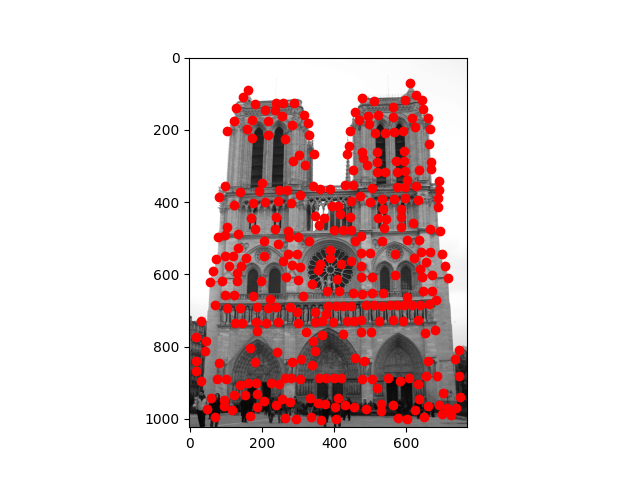
\includegraphics[width=0.75\textwidth]{images/notre_dame_figure_1_points.png} % adjust the width as needed
    \caption{Notre Dame Image 1 Interest Points}
    \label{fig:n_dame_1}
\end{figure}

\begin{figure}[H] % place the figure here if possible
    \centering
    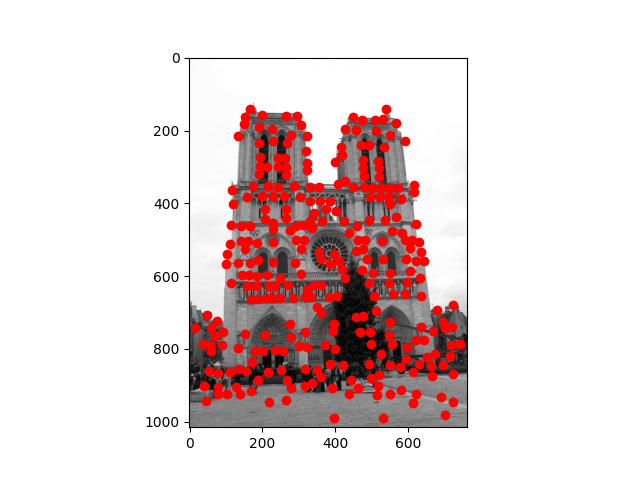
\includegraphics[width=0.75\textwidth]{images/notre_dame_figure_2_points.png} % adjust the width as needed
    \caption{Notre Dame Image 2 Interest Points}
    \label{fig:n_dame_2}
\end{figure}

\begin{figure}[H] % place the figure here if possible
    \centering
    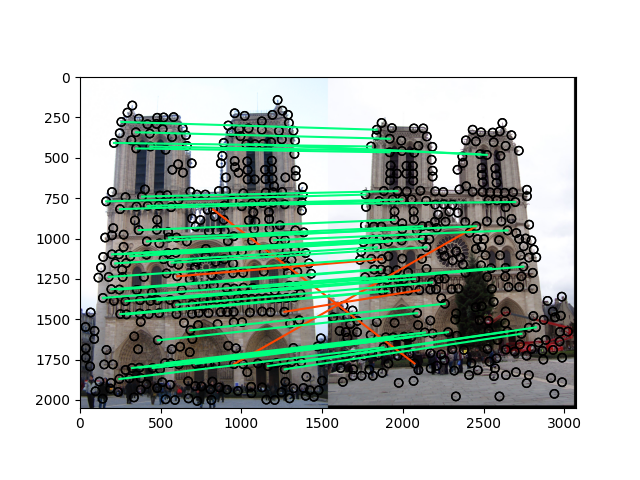
\includegraphics[width=\textwidth]{images/notre_dame_matches.png} % adjust the width as needed
    \caption{Notre Dame Matches}
    \label{fig:n_dame_match}
\end{figure}

\subsection{Mount Rushmore}
\begin{itemize}
    \item Image 1 - Number of interest points: 572
    \item Image 2 - Number of interest points: 700
    \item Matches: 249
    \item Accuracy on 50 most confident: 100\%
    \item Accuracy on 100 most confident: 83\%
    \item Accuracy on all matches: 40\%
\end{itemize}

\begin{figure}[H] % place the figure here if possible
    \centering
    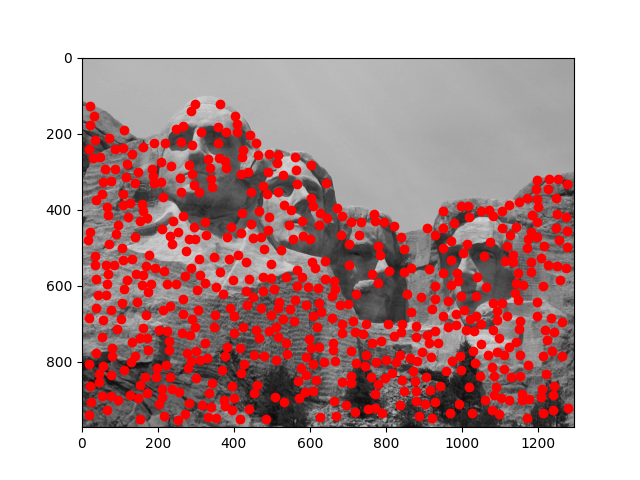
\includegraphics[width=0.75\textwidth]{images/mount_rushmore_figure_1_points.png} % adjust the width as needed
    \caption{Mount Rushmore Image 1 Interest Points}
    \label{fig:m_rushmore_1}
\end{figure}
\begin{figure}[H]
    \centering
    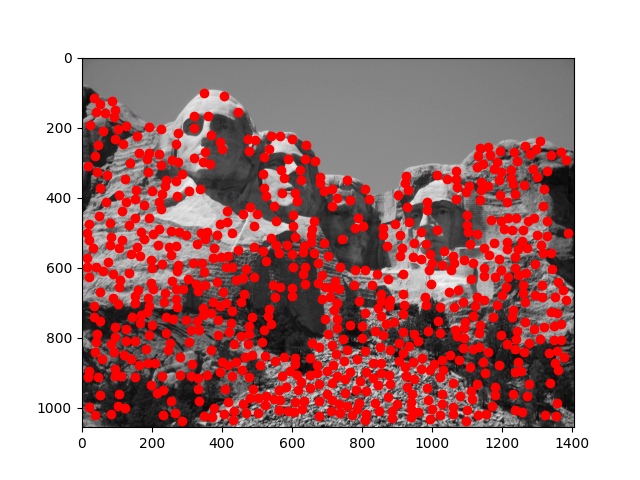
\includegraphics[width=0.75\textwidth]{images/mount_rushmore_figure_2_points.png} % adjust the width as needed
    \caption{Mount Rushmore Image 2 Interest Points}
    \label{fig:m_rushmore_2}
\end{figure}
\begin{figure}[H]
    \centering
    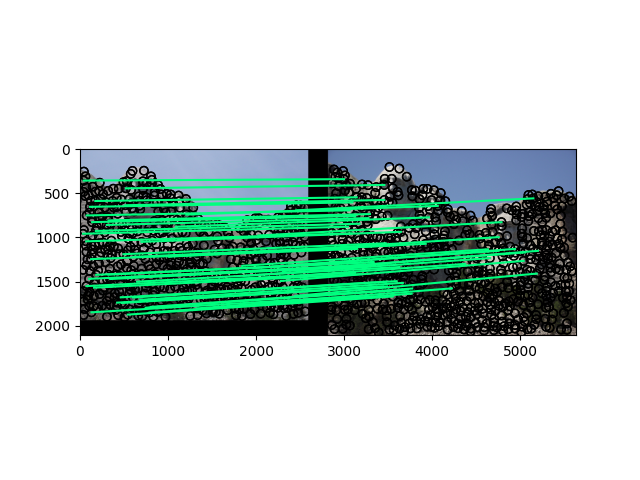
\includegraphics[width=\textwidth]{images/mount_rushmore_matches.png} % adjust the width as needed
    \caption{Mount Rushmore Matches}
    \label{fig:m_rushmore_match}
\end{figure}

\subsection{Episcopal Gaudi}
\begin{itemize}
    \item Image 1 - Number of interest points: 173
    \item Image 2 - Number of interest points: 543
    \item Matches: 62
    \item Accuracy on 50 most confident: 6\%
    \item Accuracy on all matches: 9\%
\end{itemize}

\begin{figure}[H] % place the figure here if possible
    \centering
    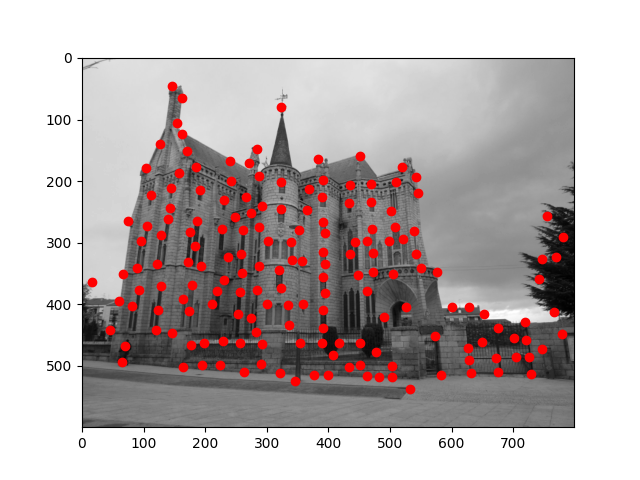
\includegraphics[width=0.75\textwidth]{images/episcopal_gaudi_figure_1_points.png} % adjust the width as needed
    \caption{Episcopal Gaudi Image 1 Interest Points}
    \label{fig:e_gaudi_1}
\end{figure}
\begin{figure}[H]
    \centering
    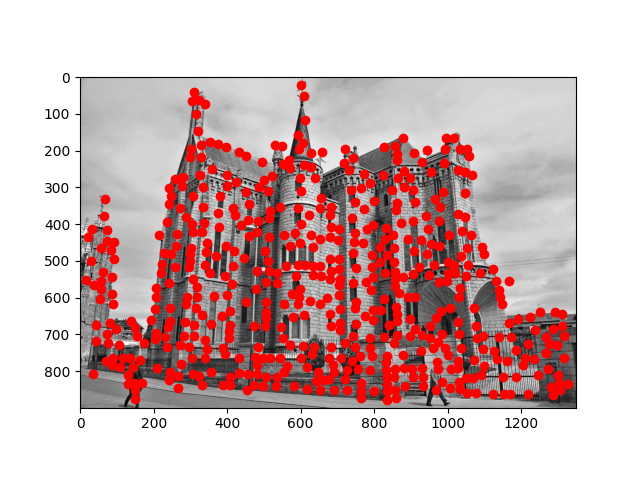
\includegraphics[width=0.75\textwidth]{images/episcopal_gaudi_figure_2_points.png} % adjust the width as needed
    \caption{Episcopal Gaudi Image 2 Interest Points}
    \label{fig:e_gaudi_2}
\end{figure}
\begin{figure}[H]
    \centering
    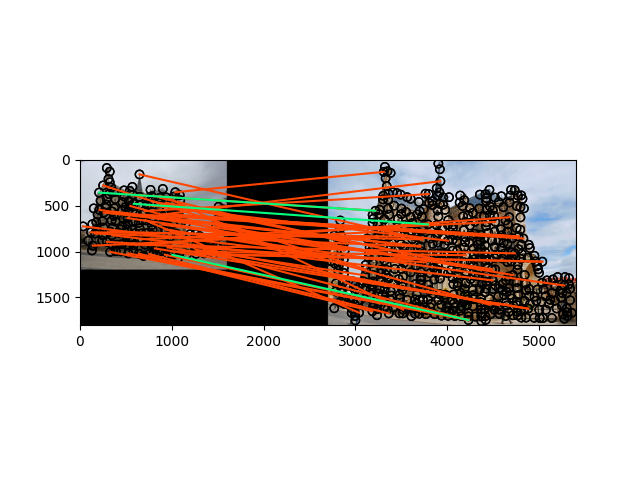
\includegraphics[width=\textwidth]{images/episcopal_gaudi_matches.png} % adjust the width as needed
    \caption{Episcopal Gaudi Matches}
    \label{fig:e_gaudi_match}
\end{figure}

\subsection{Analysis}
The key point match accuracy performs incredibly well on Notre Dame and Mount Rushmore, but very poorly on Episcopal Gaudi.

This makes sense since Episcopal Gaudi's Figure 1 and Figure 2 differ significantly. Particularily, the Figure 2 is much more crisp and sharp. Thus the number of interest points is much higher in Figure 2 as the corners are easier to detect. Furthermore, the sizes of the images are also significantly different. Figure 1 is significantly smaller than figure 2 (compared to the relative sizes of figure 1 compared to figure 2 for Notre Dame and Mount Rushmore). I believe that multi-scale keypoint detection and multi-scale feature generation could help improve the accuracy of the matches for Episcopal Gaudi.

The interest points for Notre Dame and Mount Rushmore look correct. For the Notre Dame, the corners (such at the top most right and left corners) are captured well. For Mount Rushmore, the corners of the faces (such as the nose tisp) are captured well. The matches also look correct. Something interesting is that Mount Rushmore Figure 2 has many more points than Figure 1, due to the pile of rocks in the bottom. However, these points don't get matched, which demonstrates good performance of the feature detection and matching algorithms.

In class, we learned that for feature detection, we can either add a $1$ to the bins, or the $magnitude$. I noticed that when adding magnitude, the performance actually became worse. I also tried scaling the magnitude before adding it to the bin. For the scaling factor, I used a 16x16 Gaussian kernel. As a result, the points closer to the center point would contribute a higher magnitude to their respective bins, and vice versa. This also resulted in worse performance. I believe that the reason for this is that the magnitude of the gradient is not as important as the direction of the gradient for feature detection.

\end{document}